%!TEX root = TheCourse.tex

\part{Descriptive Statistics}

% -----------------------------------------------------------------------------
% Section 1: Introduction
% -----------------------------------------------------------------------------
\section{What is Descriptive Statistics?}
\begin{frame}{Why Statistics for EEE?}
\only<article>{
    Welcome to the first module of this course: Descriptive Statistics. }   
    As Electrical Engineers, you deal with \textbf{signals} and \textbf{systems}. 
    \only<article>{
    Up until now, much of your engineering education has likely lived in the \lq Ideal World\rq . In that world, a $100\,\Omega$ resistor provides exactly $100\,\Omega$ of resistance, a $5\text{V}$ source delivers exactly $5.000\text{V}$, and Ohm's Law ($V=IR$) works with absolute, deterministic perfection.

    Unfortunately, the real world is messy.  When you open a batch of physical resistors, you will find they actually measure $98\,\Omega$, $101\,\Omega$, or $103\,\Omega$ due to manufacturing tolerances. When you measure a voltage across a sensor, thermal fluctuations will cause the reading to jitter. In electrical engineering, this uncertainty is not a mistake—it is an unavoidable physical reality.

This module is about learning the mathematical vocabulary to describe that reality. Descriptive statistics provides us with the tools to take large, messy sets of real-world data and extract meaningful engineering insights. 

    Over the next few pages, we will cover two main concepts:
    \begin{itemize}
        \item \textbf{Measures of Central Tendency:} How to find the \lq Signal\rq\ hiding in the data (using the Mean, Median, and Mode).
        \item \textbf{Measures of Dispersion:} How to quantify the \lq Noise\rq\ or uncertainty around that signal (using Variance and Standard Deviation).
    \end{itemize}

By the end of this section, you will not just be able to calculate an average; you will understand how to use these metrics to assess component reliability, evaluate system tolerances, and make informed engineering decisions. We will also introduce standard Python libraries (\texttt{NumPy} and \texttt{SciPy}) so you can handle large datasets just as you would in industry.

To illustrate the point:
}
 \only<presentation>{\vspace{0.5cm}}
    \begin{itemize}
        \item \textbf{The Ideal World:} $V = IR$. A perfect resistor has exactly $100\,\Omega$ resistance.
        \item \textbf{The Real World:} A resistor has a tolerance (e.g., $100 \pm 5\,\Omega$). Thermal noise introduces random fluctuations in voltage.
    \end{itemize}
    \only<presentation>{\vspace{0.5cm}}
        \begin{block}{The Goal}
        Statistics allows us to quantify this uncertainty, distinguish the \textbf{signal} from the \textbf{noise}, and build reliable systems from imperfect components.
    \end{block}
\end{frame}

\section{Population vs Sample}

\only<article>{
It is crucial to distinguish between \textbf{parameters}, which describe an entire \emph{population}, and \textbf{statistics}, which describe a \emph{sample} taken from that population.
}

\begin{frame}{Key Definitions: Population vs. Sample}
    \begin{columns}
        \column{0.48\textwidth}
        \begin{definition}[Population]
            The entire set of items/individuals of interest.
            \begin{itemize}
                \item Example: \textit{Every} capacitor produced by a factory in 2025.
                \item Measures are called \textbf{Parameters} (e.g., population mean, $\mu$).
            \end{itemize}
        \end{definition}

        \column{0.48\textwidth}
        \begin{definition}[Sample]
            A subset of the population selected for analysis.
            \begin{itemize}
                \item Example: A random batch of 50 capacitors tested for failure.
                \item Measures are called \textbf{Statistics} (e.g., sample mean, $\bar{x}$).
            \end{itemize}
        \end{definition}
    \end{columns}
    
    \only<article>{
        \vspace{0.3cm}
        \textbf{Example:} If we are interested in the average height of all students at the University of Manchester (the \emph{parameter}), we might statistically estimate this by measuring a \emph{sample} of students sitting in The Place at 12:00 on a Monday.

\subsection{Why do we sample in Engineering?} 
        In pure mathematics, it is sometimes possible to measure an entire population. In electrical engineering, this is often impossible due to time, cost, or the nature of the test. If a quality control test is \textbf{destructive} (for example, applying overvoltage to a capacitor until it bursts to find its ultimate failure point), testing the entire population would leave you with zero product to sell! Therefore, engineers are forced to test a small, representative sample and use statistics to infer the safety parameters of the remaining batch.
    }
\only<presentation>{\vspace{0.5cm} \centering}
%
    {\emph{In this course, we mostly calculate Statistics to estimate Parameters.}\par}
    
\end{frame}

\subsection{Representative Sample}
\begin{frame}[allowframebreaks]{Representative Sample}
    To draw valid conclusions about a population, our sample must be fair.
    \only<article>{By fair we mean not subject to any bias in the way the data is collected. The formulas we use in statistics carry a dangerous underlying assumption: they blindly assume that your sample perfectly reflects the wider population. If your sample does not, every mean, variance, and standard deviation you calculate will be mathematically flawless, but practically useless.}  

    \begin{definition}[Representative Sample]
        A \alert{representative sample} is a subset that accurately reflects the characteristics of the larger \textbf{population}.
    \end{definition}
   \only<presentation>{ \vspace{0.2cm}}

       \structure{The Goal: Randomness}
            To be representative, samples are usually collected randomly.         
          
            
            \begin{definition}[Simple Random Sample] Every member of the population has an \textbf{equal chance} of being selected.
               
        \end{definition}
        To achieve this we have to remove human choice and systematic errors. 
        \only<article>{In casual English, \lq random\rq\ often just means \lq haphazard\rq . If a manager tells an engineer to \lq go to the warehouse and pick 50 random power supplies for testing\rq , the engineer will walk in, go to the nearest pallet, and pull 50 boxes from eye level.  This is \textbf{not} a Simple Random Sample. The boxes at the back of the warehouse, or on the top shelf, had a 0\% chance of being selected. If a forklift damaged the boxes near the door, your sample is now heavily biased.
    Creating a true Simple Random Sample (SRS) in an engineering environment requires removing human choice entirely. It is a strict, three-step process:

    \begin{recipe}[Generating a Simple Random Sample]
        \begin{enumerate}
            \item \textbf{Identify and Enumerate:} Define the absolute boundary of your population (e.g., a specific batch of 5,000 microcontrollers) and ensure every single unit has a unique identifier, such as a serial number from $1$ to $N$.
            \item \textbf{Algorithmic Selection:} Do not pick items manually. Instead, use a computerized Random Number Generator (such as \texttt{numpy.random.choice()} in Python) to draw your target sample size ($n$) from the pool of available IDs. 
            \item \textbf{Blind Retrieval:} The engineer must physically extract those \textit{exact} serial numbers for the test bench. You must explicitly ignore how physically convenient or inconvenient they are to reach in the warehouse. 
        \end{enumerate}
    \end{recipe}
    
    This algorithmic approach is the only physical way to guarantee that every component has an exactly equal and independent chance of being tested, thereby protecting your statistics from human bias.
}

        \begin{block}{The Pitfall: Bias}
            \textbf{Bias} occurs when the sample systematically favours certain outcomes.    \only<article>{This will mean certain outcomes are more likely than others, destroying the assumption of randomness.  For example, suppose a quality assurance team decides to test the reliability of microchips. For convenience, they test only the first 100 chips produced right after the machines are turned on at 8:00 AM. The issues with this is that this sample completely ignores the reality of the manufacturing floor. Machines heat up, calibration drifts, and operators experience fatigue as the day progresses. By only sampling the \lq fresh\rq\ morning batch, the engineers are systematically ignoring defects caused by machine overheating at 4:00 PM. The Mathematical Consequence of this bias, is that any statistics calculated from this sample (like the sample mean failure rate, $\bar{x}$) will artificially underestimate the true population parameter ($\mu$). You can execute the mathematics perfectly in Python, but because the sample was biased, the final engineering conclusion will be dangerously wrong.}
           \only<presentation>{
            \begin{itemize}
                \item \textit{Example:} Testing only the first 100 chips produced in the morning.
                \item \textit{Issue:} This ignores defects caused by machine overheating later in the day.
                \item \textit{Consequence:} Your failure rate is underestimated. 
            \end{itemize}
            }
        \end{block}
\end{frame}






\subsubsection{Discussion: Is this Representative?}
\begin{frame}[allowframebreaks]{Discussion: Is this Representative?}


\begin{example}[The Solar Engineering]
Scenario:
    An engineering team is designing a new solar power inverter. To test its reliability, they install 50 prototype units on rooftops in \textbf{Manchester, UK} and monitor them for a year. 
    
    The data shows a 99.8\% reliability rate. The team concludes the inverter is ready for a global rollout, including markets in \textbf{Dubai} and \textbf{Arizona}.
    
    \structure{Question:}
        Is this sample representative of the global operating environment? 
        \begin{itemize}
            \item Why or why not?
            \item What variables might be missing from the sample?
        \end{itemize}
\end{example}



    \pause % This command hides the answer until you click next

\begin{solution}[The Problem: Environmental Bias]
        \textbf{No.} The sample is biased towards a cool, cloudy climate.
        \begin{itemize}
            \item \textbf{Missing Variable:} Extreme heat ($>40^\circ$C) effectively derates electronics and stresses cooling systems.
            \item \textbf{Consequence:} High failure rates possible in hot climates.
        \end{itemize}
    \end{solution}
\end{frame}

\subsection{The Problem of \lq Luck\rq\ (Sampling Error)}

\begin{frame}[allowframebreaks]{The Problem of \lq Luck\rq\ (Sampling Error)}
    Even if our sample is perfectly random and representative (no bias), it is still a subset. By pure chance, we might pick slightly more \lq high\rq\ values than \lq low\rq\ values.

    \begin{definition}[Sampling Variation (Random Error)]
        \alert{Random error} is the difference between the sample statistic ($\bar{x}$) and the true \textbf{population parameter} ($\mu$) caused purely by chance.
    \end{definition}

    \begin{example}
        You flip a fair coin 10 times. You \textit{should} get 5 Heads.
        \begin{itemize}
            \item \textbf{Result:} You get 8 Heads.
            \item \textbf{Is the coin biased?} Probably not. You just had \lq bad luck\rq\ (random variation) in your small sample.
        \end{itemize}
    \end{example}

    \only<article>{
        If you were to flip the coin 100 or 1,000 times, would you expect the sample mean ($\bar{x}$) to approach the true population mean ($\mu$)? The answer is yes. In fact, the standard error between $\bar{x}$ and $\mu$ shrinks proportionally to $1/\sqrt{n}$, where $n$ is your sample size. This is a fundamental concept known as the \textbf{Law of Large Numbers}.

        In the Probability section later in this course, we will return to this exact scenario and mathematically calculate the precise chance of getting 8 heads from 10 fair coin flips. 
        
        So, how do we handle this unavoidable uncertainty when reporting our statistics to other engineers? Instead of providing a single, fragile number, we provide a range. This naturally brings us to our next topic: Confidence Intervals.
    }

    \begin{block}{The Solution: Confidence Intervals} 
        
        \only<article>{
            When you hand a datasheet to another engineer, providing a single point estimate (like $\bar{x} = 5.0\text{V}$) is dangerous because it hides the uncertainty of your small sample. Instead, we construct a \textbf{Confidence Interval (CI)}. 
            
            A CI provides a range of plausible values for the true population parameter, explicitly communicating the margin of error. 
        }
        
        Because of this variation, we rarely state a single number. Instead, we calculate a range:
        \[ \text{\lq The voltage is } 5.0\text{V} \pm 0.1\text{V with 95\% confidence.\rq} \]
        
        \only<article>{
            \textit{What does 95\% confidence mean?} It means that if we were to repeat our sampling process 100 times, we would expect 95 of those calculated intervals to successfully capture the true, underlying population average.
        }
    \end{block}
    
    \begin{block}{Key Property: Sample Size}
        \only<presentation>{
            Unlike Bias, random error \textbf{decreases} as the sample size ($n$) increases.
            \\ \small \textit{(Law of Large Numbers)}
        }
        
        \only<article>{
            There is a fundamental difference between Bias and Random Error. If your sampling method is biased (e.g., testing only the top shelf of the warehouse), testing 10,000 units instead of 10 will not help you; it will just give you a very precise, entirely wrong number. 

            However, if your sample is truly random, you can shrink your random error simply by testing more units. As sample size ($n$) increases, the Confidence Interval becomes narrower. In engineering design, this creates a direct, real-world trade-off: the statistical precision of your data versus the financial cost of testing more components.
        }
    \end{block}
\end{frame}

%------%

\subsection{Ethics in Statistics: The \lq P-Hacking\rq\ Problem}

\begin{frame}[allowframebreaks]{Ethics in Statistics: The \lq P-Hacking\rq\ Problem}
    Since \lq bad luck\rq\ (random variation) happens, can we exploit it?
    
    \only<article>{
        We just established that random variation (sampling error) is an unavoidable physical reality. Because this variation exists, a dangerous question arises: if we test something enough times, can we weaponise that randomness to get the result we want?
    }
    
    \begin{example}[The Unethical Engineer]
        An engineer wants to prove a new battery lasts longer.
        \begin{itemize}
            \item They run \textbf{100 separate small experiments}.
            \item In 95 cases, the new battery is no better than the old one.
            \item In 5 cases, by pure random chance, the new battery performs amazingly.
            \item \textbf{Action:} They publish \emph{only} the 5 \lq successful\rq\ results and hide the rest.
        \end{itemize}
    \end{example}

    \begin{block}{This is P-Hacking (Data Dredging)}
        
        \only<presentation>{
            Technically, the data isn't \lq fake\rq ; the measurements really happened.
            However, omitting the failures distorts the probability reality. 
            \vspace{0.2cm}
            
            \textbf{Rule:} You must report \textbf{all} attempts, not just the ones that fit your desired conclusion.
        }
        
        \only<article>{
            \textbf{The Math Behind the Fraud:} Why did 5 batteries perform amazingly? Recall the concept of 95\% confidence. If you test a completely average, unimproved battery 100 times, statistical theory dictates that around 5\% of those tests will yield extreme outlier results purely by chance. The engineer hasn't invented a better battery; they have simply captured 5 instances of positive statistical noise.
            
            \vspace{0.2cm}
            \textbf{The Ethical Breach:} This practice is known as \textbf{p-hacking} or \textbf{data dredging}. The most insidious part of this fraud is that the data in those 5 reports isn't technically \lq fake\rq—the multimeter really did read those high values. However, by intentionally omitting the 95 failed tests, the engineer has completely distorted the reality of the component.
            
            \vspace{0.2cm}
            \textbf{The Engineering Consequence:} If a company bases a product rollout on those 5 cherry-picked reports, the batteries will immediately revert to their true mean in the real world. If those batteries are in consumer electronics, it causes mass recalls. If they are in medical devices or aerospace systems, it costs lives. 
            
            \vspace{0.2cm}
            \textit{The Golden Rule of Statistical Ethics:} You must report \textbf{all} experimental attempts and data points, not just the ones that fit your desired conclusion or make your design look good.
        }
    \end{block}
\end{frame}

% -----------------------------------------------------------------------------
% Section 2: Data Types
% -----------------------------------------------------------------------------
\section{Types of Data}

\only<article>{
    We have so far discussed the difference between statistics of a sample and parameters of the population. Next, we will briefly discuss the sources of engineering data and how we classify it. 
    
    Understanding your data type is the crucial first step before writing any Python code or applying any formulas. Applying the wrong statistical tool to the wrong data type will yield mathematically flawless but practically nonsensical results.
}

\subsection{Sources of data}  % Moved OUTSIDE the frame for safety
\begin{frame}{Where does Data come from?}
    \begin{definition}[Data]
        \alert{Data} is the set of observations or measurements we collect.
    \end{definition}
  
    In Engineering, it comes from two main sources:

    \begin{columns}[T]
        \column{0.48\textwidth}
        \begin{block}{\only<presentation>{1. }Finite \textbf{Population}}
            \only<presentation>{
                A fixed group of existing items.
                \begin{itemize}
                    \item \textbf{Example:} A batch of 500 resistors in a box.
                    \item \textbf{Goal:} Characterise this specific batch.
                \end{itemize}
            }
            \only<article>{
                This represents a physical, countable group of existing items. In EEE, this usually relates to \textbf{Quality Assurance (QA)} and hardware manufacturing. For example, characterising a specific batch of 500 resistors to ensure they meet a 5\% tolerance threshold. The goal is to evaluate the present state of this specific batch.
            }
        \end{block}

        \column{0.48\textwidth}
        \begin{block}{\only<presentation>{2. }Ongoing Process}
            \only<presentation>{
                A system generating data over time.
                \begin{itemize}
                    \item \textbf{Example:} Voltage noise readings from a sensor.
                    \item \textbf{Goal:} Predict the system's future behaviour.
                \end{itemize}
            }
            \only<article>{
                This represents a system that generates an infinite stream of data over time. In EEE, this relates to \textbf{Signal Processing} and system monitoring. For example, measuring the thermal noise on a communication channel. The goal here is not just to characterise the past, but to model the process so you can predict and filter out future noise.
            }
        \end{block}
    \end{columns}

    \only<presentation>{\vspace{0.5cm}}
    
    % Grouped the centering so it doesn't break future slides
    {\centering \textit{In both cases, we use \textbf{samples} (small datasets) to estimate the properties of the whole.}\par}
    
\end{frame}

\subsection{Classifying Data}
\begin{frame}{Classifying Data}
    Data generally falls into two broad categories:
    \only<presentation>{\vspace{0.5cm}}
    
    \begin{enumerate}
        \item \textbf{Qualitative (Categorical):} Non-numerical descriptions.
        \begin{itemize}
            \item Examples: Component colour codes, Pass/Fail status.
        \end{itemize}
        \only<presentation>{\vspace{0.3cm}}
        
        \item \textbf{Quantitative (Numerical):} Measured or counted values.
        \begin{itemize}
            \item This is our main focus in EEE.
            \item Further split into \textbf{Discrete} and \textbf{Continuous}.
        \end{itemize}
    \end{enumerate}
    
    \only<article>{
        \textbf{Why does this distinction matter?} \\
        Because mathematics is blind. A computer will happily let you assign the number \lq 1\rq\ to a Red wire and \lq 2\rq\ to a Blue wire, and then use \texttt{numpy.mean()} to tell you that the \lq average\rq\ wire is 1.5. This is mathematically valid but practically absurd. Qualitative data requires you to count frequencies (the Mode), while Quantitative data allows you to perform true arithmetic (the Mean and Variance). These ideas of mean, mode and variance will be introduced in the next section.
    }
\end{frame}

\subsubsection{Discrete vs. Continuous Data}

\only<article>{As stated above, quantitative data can be either \emph{discrete} or \emph{continuous}. Below we summarise the difference.}

\begin{frame}{Discrete vs. Continuous Data}
    \begin{columns}[T]
        \column{0.5\textwidth}
        \textbf{1. Discrete Data}
        \begin{itemize}
            \item Countable values (integers).
            \item No intermediate values exist.
            \item \textbf{EEE Examples:}
            \begin{itemize}
                \item Number of packets lost in transmission.
                \item Number of electrons (at quantum scale).
                \item Digital logic levels (0 or 1).
            \end{itemize}
        \end{itemize}

        \column{0.5\textwidth}
        \textbf{2. Continuous Data}
        \begin{itemize}
            \item Measurable values (real numbers).
            \item Can take any value within a range.
            \item \textbf{EEE Examples:}
            \begin{itemize}
                \item Voltage across a capacitor.
                \item Current in a wire.
                \item Signal propagation delay.
            \end{itemize}
        \end{itemize}
    \end{columns}
    
    \only<article>{
        \vspace{0.3cm}
        \textbf{The Digital Illusion (A Warning for EEEs)} \\
        As electrical engineers working with microcontrollers, you must be careful not to confuse physical reality with digital representation. A voltage across a capacitor is a \textbf{continuous} physical property—it smoothly transitions through infinite microscopic values as it charges.  However, when you measure that voltage using an Analog-to-Digital Converter (ADC) on an Arduino or Raspberry Pi, the ADC \lq quantises\rq\ that voltage into discrete digital steps (e.g., integers from $0$ to $1023$ for a 10-bit ADC). Therefore, while the physical signal in the copper trace is continuous, the dataset you end up analysing in Python is technically \textbf{discrete}.
    }
\end{frame}

% -----------------------------------------------------------------------------
% Section 3: Measures of Location
% -----------------------------------------------------------------------------
\section{Measures of Central Tendency}

\begin{frame}{Measures of Central Tendency}
    \only<article>{
        So far, we have explained the difference between a sample and an entire population, and the types of data we will encounter. Next, we consider how to mathematically describe and compare different datasets.
    }
    
    We often want to summarise a dataset with a single value that represents the \textbf{centre} or \textbf{location} of the data.
    
    \only<presentation>{\vspace{0.5cm}}

    The three most common measures are:
    \begin{enumerate}
        \item \textbf{Mean:} The arithmetic average.
        \item \textbf{Median:} The middle value.
        \item \textbf{Mode:} The most frequent value.
    \end{enumerate}
\end{frame}

\subsection{Arithmetic Mean}
\begin{frame}{1. The Arithmetic Mean}
    The mean is the most common measure of centre. It is the sum of all values divided by the number of observations.

    \begin{definition}[Sample Mean ($\bar{x}$)]
        For a sample of size $n$ with values $x_1, x_2, \dots, x_n$:
        \begin{equation}
            \bar{x} = \frac{1}{n} \sum_{i=1}^{n} x_i
        \end{equation}
    \end{definition}
    
    \begin{recipe}[Calculating the Mean]
        \begin{enumerate}
            \item Sum all the values.
            \item Divide by the number of values.
        \end{enumerate}
    \end{recipe}

    \textbf{Note:}
    \begin{itemize}
        \item For a \textbf{Population}, we use the symbol $\mu$.
        \item The mean is highly sensitive to \textbf{outliers} (extreme values).
    \end{itemize}
\end{frame}

\subsection{Median}
\begin{frame}{2. The Median}
    \begin{definition}[Median]
        The \alert{median} is the middle value when the data is ordered from smallest to largest.
    \end{definition}
    
    \begin{recipe}[Calculating the Median]
        \begin{enumerate}
            \item Sort the data: $x_{(1)} \le x_{(2)} \le \dots \le x_{(n)}$.
            \item Find the position:
            \begin{itemize}
                \item If $n$ is \textbf{odd}: The median is the exact middle number.
                \item If $n$ is \textbf{even}: The median is the average of the two middle numbers.
            \end{itemize}
        \end{enumerate}
    \end{recipe}
    
    \only<presentation>{\vspace{0.3cm}}
    \textit{The median is \textbf{robust} (less affected by outliers).}
\end{frame}

\subsection{Mode}
\begin{frame}{3. The Mode}
    \begin{definition}[Mode]
        The \alert{mode} is the value that occurs most frequently in the dataset.
    \end{definition}

    \begin{recipe}[Calculating the Mode]
        \begin{enumerate}
            \item List all unique values in the dataset.
            \item Count the frequency (number of occurrences) for each value.
            \item Identify the value(s) with the highest frequency.
            \begin{itemize}
                \item If multiple values share the highest count, the data is \textbf{multimodal}.
                \item If all values appear only once, there is \textbf{no mode}.
            \end{itemize}
        \end{enumerate}
    \end{recipe}

    \begin{itemize}
        \item Useful for Qualitative data (e.g., \lq The most common failure mode is overheating\rq).
    \end{itemize}
\end{frame}

% -----------------------------------------------------------------------------
% Section 4: Worked Example
% -----------------------------------------------------------------------------
\subsection{Worked Example}

\begin{frame}[allowframebreaks]{Worked Example: Signal Latency}
    \begin{example}[Network Router Latency]
        An engineer measures the latency (in ms) of 5 packets passing through a network router:
        \[ \text{Data:} \quad 12, \quad 15, \quad 12, \quad 200, \quad 14 \]
        
        \structure{Questions:}
        \begin{enumerate}
            \item Calculate the mean, median, and mode.
            \item Draw an engineering conclusion: Which measure best represents the network's typical performance?
        \end{enumerate}
    \end{example}
    
    \pause
    
    \begin{solution}
        \textbf{Part 1: Calculations}
        \begin{itemize}
            \item \textbf{Mean:} 
            \[ \bar{x} = \frac{12+15+12+200+14}{5} = \frac{253}{5} = \textbf{50.6 ms} \]
            \item \textbf{Median:} Sort the data: $12, 12, \mathbf{14}, 15, 200$. 
            \[ \text{Median} = \textbf{14 ms} \]
            \item \textbf{Mode:} The most frequent value is \textbf{12 ms}.
        \end{itemize}
        \end{solution}
        \vspace{0.3cm}
        \begin{solution}
        \textbf{Part 2: Interpretation}
        \begin{itemize}
            \item \textbf{Mean (50.6 ms):} Heavily skewed by the single outlier (200 ms). This metric falsely suggests the entire network is slow, which is only true for 1 packet (perhaps due to a temporary buffer spike).
            \item \textbf{Median (14 ms):} Gives a much more accurate representation of the \lq typical\rq\ performance the user will experience.
        \end{itemize}
    \end{solution}
    
    \begin{block}{Key Takeaway}
        Always look at the data distribution. If the data is skewed (like network latency, income, or component lifespans often are), the \textbf{median} is a much safer measure of the centre than the \textbf{mean}.
    \end{block}
    \only<article>{
    \subsection{Why does this happen? The Physics of the Mean} 
    Think of the \textbf{mean} as the physical \textit{centre of mass} of your dataset. If you imagine placing your data points on a seesaw, the mean is the exact fulcrum point required to make the seesaw balance perfectly flat. 
    
    In our router example, four of the packets are clustered tightly together between 12\,ms and 15\,ms, but the 200\,ms outlier is sitting incredibly far down the right-hand side of the seesaw. To prevent the seesaw from tipping over, the fulcrum (the mean) must be dragged drastically to the right—all the way to 50.6\,ms. In statistics, this dragging effect is called \textbf{skew}.
    
    
    
    The \textbf{median}, on the other hand, does not care about physical distance or mass; it only cares about \textit{rank order}. Once the data is sorted, the median simply points to the item exactly in the middle of the queue. 
    
    Look at our sorted data again: $12, 12, \mathbf{14}, 15, \text{outlier}$. 
    Whether that final outlier is 20\,ms, 200\,ms, or 2,000,000\,ms, the middle packet will always be 14\,ms. This mathematical property makes the median incredibly \textbf{robust}. In real-world engineering, where sensor glitches, network buffer spikes, or manufacturing anomalies occasionally produce wildly extreme numbers, the median protects your analysis from being ruined by a single bad data point.
}
\end{frame}

\only<presentation>{
\begin{frame}{Interactive Demonstration}
    \structure{The Pull of the Outlier}
    
    Let's look at how the Mean and Median react in real-time when we introduce an extreme network delay.
    
    \vspace{1cm}
    \centering
    % This creates a beautiful Beamer-styled button
    % It tells the OS to run the python file located in the same folder as your PDF
    \href{run:./code/run_MeanVersusMedium.command}{\beamerbutton{\Large Launch Python Simulation}}
    
    \vspace{1cm}
    \textit{(Note: This will open an external interactive Matplotlib window.)}
\end{frame}
}

\section{Python to the Rescue}
\subsection{Setting up VS code for python}
\begin{frame}[fragile]{Our Python Environment: Keeping it Standard}
    \only<article>{
        In this course we will show how to do large calculations with Python. To avoid the dreaded \lq it works on my machine!\rq\ excuse and completely eliminate version conflicts, we are strictly aligning our Python tools with your \textbf{EEEN11202} module.
    }

    \begin{block}{The Engineering Stack}
        \begin{itemize}
            \item \textbf{Editor:} Visual Studio Code (VSCode)
            \only<article>{
                \\ \textit{VS Code is a lightweight, wildly popular code editor. Unlike heavy IDEs, it is essentially a highly customisable text editor that becomes powerful through extensions. Download it directly from code.visualstudio.com.}
            }
            \item \textbf{Environment:} Devcontainers (Isolated and reproducible)
            \only<article>{
                \\ \textit{A Devcontainer runs a tiny, invisible Linux machine inside your computer. It guarantees that every student---regardless of whether they have an M-series Mac or a Windows PC---is running the exact same version of Python with the exact same settings.}
            }
            \item \textbf{Package Manager:} \texttt{uv} (Blazing fast, modern standard)
            \only<article>{
                \\ \textit{Once inside your Devcontainer, you need to download statistical libraries. \texttt{uv} is a next-generation Python package manager written in Rust. It is blisteringly fast (often 10x to 100x faster than \texttt{pip}) and rigorously manages your project files.}
            }
        \end{itemize}
    \end{block}

   \only<presentation>{ \vspace{0.2cm}}
    \structure{Getting Ready for Statistics:}
    \only<article>{
        \\ When you boot up your EEEN11202 devcontainer for our examples, you must initialise your project space and add the statistical libraries.
        \begin{enumerate}
           \item \textbf{Verify connection:} Look at the far bottom-left corner of the VS Code window for a coloured box containing a \texttt{><} icon. 
    \\ \textit{If this box says \lq Dev Container\rq, you are safely inside the isolated Linux environment. If it does not, click the \texttt{><} icon and select \lq Reopen in Container\rq\ from the drop-down menu before running any terminal commands!}
            \item \textbf{Initialise:} Ensure you run \texttt{uv init} in the terminal first to create your configuration file.
            \item \textbf{Install libraries:} Run the command below to download our specific tools.
        \end{enumerate}
    }
    \only<presentation>{For this course we need \textit{numpy, scipy} and \textit{matplotlib}.}

    \only<presentation>{\vspace{0.1cm}}
    \insertcode{Setup}{code/SetupVS.py}

  \only<presentation>{  \vspace{0.1cm}}
    \textit{No PyCharm, no Anaconda, no conflicts. Just engineering efficiency!}
\end{frame}


\begin{frame}[fragile,allowframebreaks]{Statistics in Action: Python}
    In modern engineering, we rarely calculate statistics by hand. We leverage the power of the \textbf{SciPy Stack}, specifically \texttt{numpy} and \texttt{scipy.stats}.
    
    \only<article>{
        \subsection{Context: The \lq SciPy Stack\rq}
        
        One of the most confusing aspects for beginners is the terminology around \lq SciPy\rq . 
        \begin{itemize}
            \item \textbf{SciPy (The Library):} A specific package containing algorithms.
            \item \textbf{SciPy (The Stack):} The entire ecosystem of tools that work together.
        \end{itemize}

        In Engineering, we treat the \lq SciPy Stack\rq\ as a single cohesive toolkit, similar to how MATLAB operates. It is built as a hierarchy of layers, where each tool relies on the one below it.

        \begin{figure}[h]
            \centering
            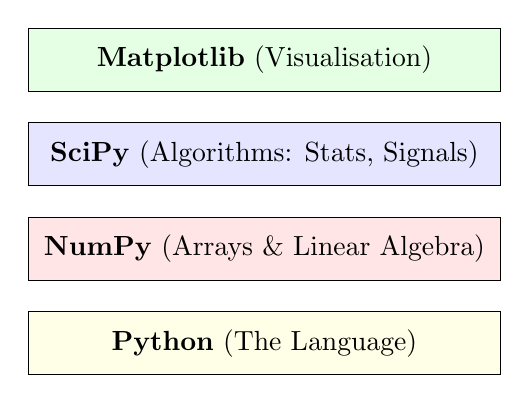
\begin{tikzpicture}[node distance=1.2cm]
                % Visualising the Stack as a Pyramid
                \node (viz) [draw, fill=green!10, minimum width=6cm, minimum height=0.8cm] {\textbf{Matplotlib} (Visualisation)};
                \node (tools) [draw, fill=blue!10, minimum width=6cm, minimum height=0.8cm, below of=viz] {\textbf{SciPy} (Algorithms: Stats, Signals)};
                \node (math) [draw, fill=red!10, minimum width=6cm, minimum height=0.8cm, below of=tools] {\textbf{NumPy} (Arrays \& Linear Algebra)};
                \node (lang) [draw, fill=yellow!10, minimum width=6cm, minimum height=0.8cm, below of=math] {\textbf{Python} (The Language)};
            \end{tikzpicture}
            \caption{The Hierarchy of the Scientific Python Ecosystem. You cannot use the top layers without the bottom ones.}
            \label{fig:scipy_stack}
        \end{figure}

        \subsection{The Key Components}
        \begin{itemize}
            \item \textbf{1. NumPy (Numerical Python):} This is the foundation. Python's built-in lists are flexible but slow. NumPy introduces the \texttt{ndarray} (n-dimensional array), which is memory-efficient and extremely fast. \textit{If you are doing math in Python, you are likely using NumPy.}
            \item \textbf{2. SciPy (Scientific Python):} This is the \lq Engine Room\rq . It assumes you already have your data in NumPy arrays. It provides the complex algorithms you would find in an engineering textbook:
            \begin{itemize}
                \item \texttt{scipy.stats}: Probability distributions and tests.
                \item \texttt{scipy.signal}: Filter design and waveforms.
                \item \texttt{scipy.optimize}: Curve fitting and minimisation.
            \end{itemize}
            \item \textbf{3. Matplotlib:} The standard library for plotting graphs. It is designed to work natively with NumPy arrays.
            \item \textbf{4. Pandas:} (Optional but common) Used for \lq Tabular Data\rq\ (like Excel sheets or CSV files). It sits on top of NumPy but provides named columns and easier data cleaning tools.
        \end{itemize}
    }

    \vspace{0.3cm}

    \begin{columns}[T]
        \begin{column}{0.48\textwidth}
            \structure{\textbf{NumPy} (The Foundation)}
            \begin{itemize}
                \item \textbf{Efficiency:} Highly optimised for $N$-dimensional arrays.
                \item \textbf{Speed:} Vectorised operations outperform standard Python loops.
                \item \textbf{Linear Algebra:} Essential for handling large datasets.
            \end{itemize}
        \end{column}
        
        \begin{column}{0.48\textwidth}
            \structure{\textbf{SciPy} (The Toolbox)}
            \begin{itemize}
                \item \textbf{scipy.stats:} Specialised functions for probability distributions (Normal, $t$-tests, $p$-values).
                \item \textbf{Fitting:} Tools to fit experimental data to mathematical models.
                \item \textbf{Integration:} Built-in solvers for complex engineering calculus.
            \end{itemize}
        \end{column}
    \end{columns}

    \vspace{0.5cm}
    \insertcode{Python Code Example: Mean, mode, medium}{code/lecture1_stats.py}
    
    \only<presentation>{
        \begin{itemize}
            \item \textbf{Imports:} We use \texttt{numpy} (standard for arrays) and \texttt{scipy.stats} (for specific statistical functions).
            \item \textbf{Efficiency:} \texttt{np.mean()} and \texttt{np.median()} are highly optimised. They run much faster than writing a loop yourself.
            \item \textbf{The \lq Mode\rq\ Trap:} Unlike mean/median, \texttt{stats.mode} returns a complex object (Value + Count).
            \item \textbf{Extraction:} We must use \texttt{.mode[0]} to pull out the actual number for printing.
        \end{itemize}
    }

    \only<article>{
        \subsection*{Code Breakdown: Calculating Averages in Python}
        
        Below is a detailed explanation of the script.
        
        \begin{itemize}
            \item \textbf{\texttt{import numpy as np}:} This imports the \textbf{NumPy} library, which is the industry standard for engineering mathematics. We alias it as \texttt{np} to save typing. It contains highly optimised code for handling arrays and matrices.
            
            \item \textbf{\texttt{from scipy import stats}:} While NumPy handles basic math, \textbf{SciPy} (Scientific Python) contains more advanced statistical tools. We need this specifically for calculating the \textit{Mode}, which NumPy does not support directly.
            
            \item \textbf{\texttt{data = [...]}:} We define our dataset as a standard Python list. Note that NumPy functions are smart enough to accept a list and convert it to an optimised array automatically.
            
            \item \textbf{\texttt{np.mean(data)} \& \texttt{np.median(data)}:} These functions calculate the location measures. They handle floating-point math automatically. If the list had an even number of elements, \texttt{np.median} would automatically interpolate the middle two values.
            
            \item \textbf{\texttt{stats.mode(data, keepdims=True)}:} This is the most complex line. 
            \begin{itemize}
                \item \texttt{keepdims=True}: This ensures the output shape matches the input, preventing warnings in newer versions of SciPy.
                \item \textbf{The Return Value:} This function does \textit{not} return a single number. It returns a \texttt{ModeResult} object containing two arrays: the mode(s) and the count(s).
            \end{itemize}

            \item \textbf{\texttt{print(f"...")}:} We use \textbf{f-strings} (formatted string literals) to insert variables directly into printed text.
            
            \item \textbf{\texttt{mode\_result.mode[0]}:} Since \texttt{mode\_result} is an object containing arrays, we cannot just print it. We access the \texttt{.mode} attribute (which is an array) and take the first element \texttt{[0]} to get the actual scalar value (e.g., \texttt{12}).
        \end{itemize}
    }
\end{frame}

\only<article>{
    \subsection{Our Interactive Mean versus Median Demo}
    Now we know a little bit about Python, we can write a simple script to experiment with outliers and illustrate the issues with skew.
    
    \insertcode{Mean versus Median Simulator}{code/MeanVersusMedian.py}
    
    This code gives you an interactive set of sliders to change the latency of 5 data packets and instantly recalculates and plots both the mean and the median.
}
% -----------------------------------------------------------------------------
% Summary
% -----------------------------------------------------------------------------
\section{Summary so far}
\begin{frame}{Summary - First Half}
    \begin{itemize}
        \item \textbf{Data Types:} Identify if your variables are Discrete (counts) or Continuous (measurements).
        \item \textbf{Notation:} $\bar{x}$ for Sample Mean, $\mu$ for Population Mean.
        \item \textbf{Central Tendency:}
        \begin{itemize}
            \item \textbf{Mean:} Mathematical centre, sensitive to outliers.
            \item \textbf{Median:} Positional centre, robust.
            \item \textbf{Mode:} Most frequent, good for categories.
        \end{itemize}
    \end{itemize}

    \vspace{0.5cm}
    \textbf{Next:} We will look at \textit{Measures of Dispersion} (Range, Variance, Standard Deviation) to understand the ``spread'' of the data.
\end{frame}






\section{Measures of Dispersion (Spread)}

\only<article>{
    So far in the previous section, we discussed how to measure the \lq average\rq\ of a dataset, but often this is not enough information and we also have to consider the \lq spread\rq\ of the data.
}

% --- SLIDE 1: The Problem with Averages ---
\subsection{Why Central Tendency isn't enough}

\begin{frame}{Why Central Tendency isn't enough}
    \begin{example}[The \lq Average\rq\ Weather]
        Consider two cities with the same Mean Yearly Temperature ($20^\circ$C).
        
        % The Ranges (The Reveal on Slide 2)
        \visible<2->{
            \begin{itemize}
                \item \textbf{\textcolor{blue}{City A (Stable):}} Ranges from $18^\circ$C to $22^\circ$C.
                \item \textbf{\textcolor{red}{City B (Extreme):}} Ranges from $-10^\circ$C to $50^\circ$C.
            \end{itemize}
        }
        
        % The Trap Question (Visible from Slide 1)
        \only<presentation>{\vspace{0.2cm}}
        \visible<1->{\structure{Question:} Would you build the same bridge or roads in both?}
    \end{example}

    % --- BEAMER ONLY: Show the graphic on slide 3 ---
    \only<presentation>{
        \visible<3>{
            \vspace{0.2cm}
            \centering
            \small An engineer needs to design for the \textbf{Extremes} (Spread).
            \vspace{0.2cm}
            
            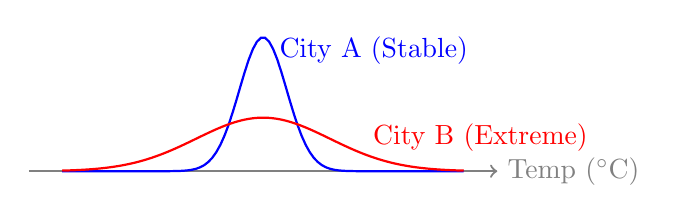
\begin{tikzpicture}[scale=0.85] 
                % Draw Axis
                \draw[->, thick, gray] (-3.5,0) -- (3.5,0) node[right] {Temp ($^\circ$C)};
                
                % Narrow Curve (Blue)
                \draw[blue, thick] plot[domain=-3:3, samples=100] (\x, {2*exp(-4*\x*\x)});
                \node[blue, right] at (0.1, 1.8) {City A (Stable)};

                % Wide Curve (Red)
                \draw[red, thick] plot[domain=-3:3, samples=100] (\x, {0.8*exp(-0.5*\x*\x)});
                \node[red, right] at (1.5, 0.5) {City B (Extreme)};
            \end{tikzpicture}
        }
    }
\end{frame}

% --- ARTICLE ONLY: A proper floating figure for the handbook ---
\only<article>{
    \begin{figure}[htbp]
        \centering
        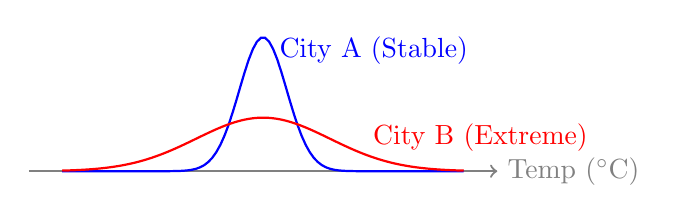
\begin{tikzpicture}[scale=0.85] 
            % Draw Axis
            \draw[->, thick, gray] (-3.5,0) -- (3.5,0) node[right] {Temp ($^\circ$C)};
            
            % Narrow Curve (Blue)
            \draw[blue, thick] plot[domain=-3:3, samples=100] (\x, {2*exp(-4*\x*\x)});
            \node[blue, right] at (0.1, 1.8) {City A (Stable)};

            % Wide Curve (Red)
            \draw[red, thick] plot[domain=-3:3, samples=100] (\x, {0.8*exp(-0.5*\x*\x)});
            \node[red, right] at (1.5, 0.5) {City B (Extreme)};
        \end{tikzpicture}
        \caption{Frequency distribution of the highest daily temperatures.}
        \label{fig:temp_spread}
    \end{figure}
Clearly we cannot use the same materials for each.    To understand why dispersion dictates design, let's look more carefully at the materials required for our two cities. Because City B has a huge temperature spread ($\Delta T = 60^\circ$C) compared to City A ($\Delta T = 4^\circ$C), the physical engineering requirements change drastically:

    \begin{itemize}
        \item \textbf{The Road Surface (Asphalt/Bitumen):} 
        Asphalt is highly temperature-sensitive. In City A, you can use a cheap, standard bitumen binder because the temperature never leaves a comfortable ambient zone. If you used that same cheap asphalt in City B, it would become soft and deform under heavy truck tires at $50^\circ$C (rutting), and it would become glass-like and shatter under impact at $-10^\circ$C. City B requires highly engineered, expensive Polymer-Modified Bitumen.
        
        \item \textbf{Thermal Expansion Joints:} 
        Most metals expand when heated. For a 100-metre steel bridge in City A, the steel will only expand by about 5 millimetres over the year. You can practically ignore it. In City B, that same steel span will expand and contract by over 70 millimetres. If you don't install massive, expensive mechanical expansion joints, the bridge will literally tear itself off its concrete foundations during the summer.
        
        \item \textbf{Concrete and Moisture (Freeze-Thaw):} 
        In City A, standard concrete is fine. In City B, the temperature drops below freezing. Any rainwater that seeps into micro-cracks in the concrete will freeze, expand, and blow the surface off the concrete (spalling). City B absolutely requires \lq air-entrained\rq\ concrete—a special mix containing millions of microscopic air bubbles to give the freezing ice room to expand.
    \end{itemize}
    
    In short: the \textit{mean} temperature tells you where to build. The \textit{dispersion} (variance) tells you how much the materials will cost.
}
\subsection{Why do we measure Spread?}

% --- BEAMER SLIDE ---
\begin{frame}{Why do we measure Spread?}
    \only<presentation>{\structure{The Danger of the \lq Average\rq}}
    
    In engineering design, the average is often a completely useless metric for safety. We must design for the extremes.

    \only<presentation>{
        \vspace{0.3cm}
        \pause % Adds a nice click-to-reveal effect during your lecture
    }

    \begin{block}{Real-World Engineering Constraints}
        \only<article>{Let's consider a few actual examples:}
        \begin{itemize}
            \item A structural beam fails at the \textbf{maximum} load, not the average load.
            \item A circuit overheats at the \textbf{peak} current, not the average current.
        \end{itemize}
    \end{block}

    \only<presentation>{
        \vspace{0.3cm}
        \pause

        \begin{alertblock}{The Meaning of Dispersion}
            \textbf{Dispersion} tells us how reliable or volatile our system is. \\
            \vspace{0.1cm}
            $\implies$ \textbf{High Dispersion = High Risk or Low Precision.}
        \end{alertblock}
    }
    
    \only<article>{
        The dispersion of our data gives us insights into the reliability and volatility of the system. If we want a highly reliable, low-risk system, we should minimise the dispersion. Of course, we can do this if we are designing a new component (or at least try!), but this is much harder to do with external variables like the weather.
    }
\end{frame}

%\subsection{Summary of dispersion measures}

\only<article>{
    Just as there are different measures of \lq average\rq, there are several measures of dispersion as well, each with its own pros and cons. Here we will focus on three commonly used measures of dispersion:
    \begin{enumerate}
        \item Range
        \item Interquartile Range (IQR)
        \item Variance and Standard Deviation
    \end{enumerate}
}


\subsection{The Range}

\begin{frame}{1. The Range}
    The simplest measure of spread.
    \[ \text{Range} = x_{max} - x_{min} \]
    
    \only<presentation>{
        \begin{block}{Weakness: Sensitivity to Outliers}
            Dataset: $\{ 1, 2, 3, 4, 5 \}$ $\rightarrow$ Range = 4. \\
            Dataset: $\{ 1, 2, 3, 4, \mathbf{100} \}$ $\rightarrow$ Range = 99.
        \end{block}
        
        The range ignores the internal structure of the data. It only cares about the two most extreme values, which might be errors.
    }
    
    \only<article>{
        The range is the most intuitive measure of dispersion, but it is also the most fragile. Because the calculation strictly relies on the absolute maximum and minimum values, a single sensor glitch or anomaly will completely destroy the metric.
        
        \begin{example}[Revisiting Network Latency]
            Recall our network router example from the previous section, where we measured five packet latencies: 
            \[ 12\text{ms}, \quad 12\text{ms}, \quad 14\text{ms}, \quad 15\text{ms}, \quad \mathbf{200\text{ms}} \]
            
            If we calculate the range of this dataset:
            \[ \text{Range} = 200\text{ms} - 12\text{ms} = \textbf{188 ms} \]
            
            \textbf{The Engineering Trap:} 
            If you report a spread of $188\text{ms}$ to your project manager, they will assume the network is incredibly volatile and unpredictable. However, we know by looking at the data that $80\%$ of the packets arrived within a tiny, highly stable $3\text{ms}$ window (between $12\text{ms}$ and $15\text{ms}$). 
            
            The range completely ignores the tight internal clustering of the data. It allows one anomalous 200ms packet to hijack the entire narrative.
        \end{example}
        
        While the range is useful for a quick \lq sanity check\rq\ of your dataset boundaries, it is rarely used for serious engineering analysis. We need statistical tools that account for \textit{every} data point, not just the extremes. This leads us to Variance and Standard Deviation.
    }
\end{frame}

\subsection{Interquartile Range (IQR)}
\begin{frame}{2. Interquartile Range (IQR)}
    If the Median is our robust \lq average\rq, the IQR is our robust \lq spread\rq. 
    It measures the range of the \textbf{middle 50\%} of your data, completely ignoring the extremes.
    
    \only<presentation>{\vspace{0.3cm}}
    
    \begin{definition}[Quartiles]
        To find the IQR, we split the sorted data into four equal quarters:
        \begin{itemize}
            \item \textbf{$Q_1$ (Lower Quartile):} The 25th percentile.
            \item \textbf{$Q_2$ (Median):} The 50th percentile.
            \item \textbf{$Q_3$ (Upper Quartile):} The 75th percentile.
        \end{itemize}
    \end{definition}
    
    \begin{block}{The IQR Formula}
        \centering
        $\text{IQR} = Q_3 - Q_1$
    \end{block}
    
    \only<presentation>{
        \vspace{0.2cm}
        \textit{By stripping away the bottom 25\% and top 25\% of the data, the IQR becomes highly immune to sensor glitches and extreme outliers.}
    }

    \only<article>{
        \vspace{0.3cm}
        \textbf{Why the IQR is an Engineering Shield} \\
        Standard Deviation and Range are easily destroyed by a single bad data point. Because the IQR explicitly throws away the highest and lowest quarters of your dataset before doing any math, it acts as a protective shield against anomalies. 
        
        \begin{example}[Calculating the IQR]
            Let's look at 7 temperature readings from a thermistor (in $^\circ\text{C}$), sorted in order. One reading is clearly a system error:
            \[ 10, \quad 12, \quad 14, \quad \mathbf{15}, \quad 17, \quad 18, \quad \mathbf{200} \]
            
            \begin{enumerate}
                \item \textbf{Find the Median ($Q_2$):} The middle value is clearly $15^\circ\text{C}$.
                \item \textbf{Find $Q_1$:} Look at the lower half of the data ($10, 12, 14$). The median of this lower half is $12^\circ\text{C}$.
                \item \textbf{Find $Q_3$:} Look at the upper half of the data ($17, 18, 200$). The median of this upper half is $18^\circ\text{C}$.
            \end{enumerate}
            
            Now, calculate the spreads:
            \begin{itemize}
                \item \textbf{The Range:} $200 - 10 = \mathbf{190^\circ\text{C}}$ \textit{(Falsely implies massive volatility)}
                \item \textbf{The IQR:} $18 - 12 = \mathbf{6^\circ\text{C}}$ \textit{(Accurately describes the typical behavior)}
            \end{itemize}
            
            The IQR correctly tells the engineer that the vast majority of the time, this system is highly stable, fluctuating within a tight $6^\circ\text{C}$ window.
        \end{example}

        \begin{block}{Visualising the IQR}
            If you ever plot a \textbf{Box Plot} (or Box-and-Whisker plot) in Python using \texttt{matplotlib.pyplot.boxplot()}, the \lq box\rq\ in the middle is drawn exactly from $Q_1$ to $Q_3$. The width of that box is your IQR!
        \end{block}
    }
\end{frame}

\subsection{The Variance}
% --- SLIDE 3: Variance Concept ---
\begin{frame}{2. The Variance ($\sigma^2$ or $s^2$)}
    How do we measure \lq average spread\rq\ using \textit{all} data points?
    %
    \only<presentation>{\textbf{The Logic:}} \only<article>{We need some measure of distance the data is from the mean hence we can think of the average square distance from the mean i.e.}
    \begin{enumerate}
        \item Find the distance of every point from the Mean: $(x_i - \bar{x})$.
        \item Square them to remove negatives: $(x_i - \bar{x})^2$.
        \item Average these squared distances.
    \end{enumerate}

    \only<presentation>{\vspace{0.5cm}}
    \textbf{Why Square?} 
    If we just added the distances $(x - \bar{x})$, the negatives would cancel the positives, summing to zero. Squaring makes everything positive.
\end{frame}

% --- SLIDE 4: Population vs Sample ---
\subsubsection{Population vs Sample}
\begin{frame}{Population vs. Sample Variance}
    This is the most common mistake in engineering statistics.
    
    \begin{columns}
        \column{0.5\textwidth}
        \textbf{Population Variance ($\sigma^2$)} \\
        Used when you have \textbf{all} the data (e.g., a census).
        \[ \sigma^2 = \frac{\sum (x - \mu)^2}{N} \]
        
        \column{0.5\textwidth}
        \textbf{Sample Variance ($s^2$)} \\
        Used when you have a \textbf{subset} (e.g., 10 sensors out of 1000).
        \[ s^2 = \frac{\sum (x - \bar{x})^2}{n-1} \]
    \end{columns}
 \only<presentation>{
    \vspace{0.5cm}
  \alert{Why $n-1$?} This is \textbf{Bessel's Correction}. It corrects for the fact that samples tend to underestimate the true spread of the population.}
\end{frame}

\only<article>{
    \subsubsection{Bessel's Correction ($n-1$)}
    Why do we divide by $n-1$ for samples? Imagine you measure the height of 5 random people. It is highly unlikely you picked the shortest person on Earth AND the tallest person on Earth. Therefore, your sample spread is likely \textit{smaller} than the true human population spread. Dividing by a smaller number ($n-1$ instead of $n$) makes the result slightly \textit{bigger}, correcting for this bias. As $n$ gets huge (e.g., 1 million), difference between $n$ and $n-1$ becomes negligible.
}

%\begin{frame}{Why divide by $n-1$? (Bessel's Correction)}
%    \begin{block}{The Problem: Bias}
%        When we calculate Sample Variance ($s^2$), we use the \textbf{Sample Mean} ($\bar{x}$) because we don't know the true \textbf{Population Mean} ($\mu$).
%        
%        \begin{itemize}
%            \item The data points are always closer to their own average ($\bar{x}$) than to the true population average ($\mu$).
%            \item Therefore, $\sum (x - \bar{x})^2$ is always \textbf{smaller} than $\sum (x - \mu)^2$.
%        \end{itemize}
%    \end{block}
%
%    \begin{example}[The Correction]
%        If we divided by $n$, our variance would be consistently \textbf{too low} (Biased).
%        
%        By dividing by \textbf{$n-1$}:
%        \begin{itemize}
%            \item We make the denominator smaller.
%            \item This makes the total result \textbf{larger}.
%            \item This "inflates" the variance just enough to remove the bias.
%        \end{itemize}
%    \end{example}
%\end{frame}

% --- SLIDE 5: Standard Deviation ---
\subsubsection{Standard Deviation}

\begin{frame}{3. Standard Deviation ($\sigma$ or $s$)}
    \textbf{The Problem with Variance:}
    If we measure length in meters (m), Variance is in meters-squared ($m^2$). This is physically confusing.
    
    \only<article>{
        \vspace{0.2cm}
        In electrical engineering, if you are measuring the output voltage of a power supply and the mean is $5\text{V}$, the variance might be calculated as $0.04\text{V}^2$. While mathematically necessary for intermediate steps, \lq volts squared\rq\ is not a helpful unit when you are trying to determine if a $5\text{V}$ logic gate is going to fry. We need a measure of spread that shares the exact same physical units as our original data and our mean.
    }
    
    \textbf{The Solution:}
    Take the square root to return to the original units.
    
    \[ s = \sqrt{s^2} = \sqrt{ \frac{\sum (x - \bar{x})^2}{n-1} } \]
    
    \begin{itemize}
        \item \textbf{High SD:} Data is spread out (Noisy, Unreliable).
        \item \textbf{Low SD:} Data is clustered near the mean (Precise, Consistent).
    \end{itemize}
    
    \only<article>{
        \vspace{0.3cm}
        \textbf{The Engineering Reality: Tolerances and Quality Control} \\
        Standard Deviation is arguably the most important statistical metric in modern manufacturing. When you buy a $1\text{k}\Omega$ resistor with a $\pm 1\%$ tolerance, the manufacturer is relying on standard deviation to guarantee that rating. 
        
        Later in the course, we will explore the \textbf{Normal Distribution} (the Bell Curve). When data follows this natural curve, Standard Deviation acts as a physical ruler for your dataset:
        
        

        \begin{itemize}
            \item Roughly \textbf{68\%} of your manufactured components will fall within \textbf{one} standard deviation ($\pm 1s$) of the mean.
            \item Roughly \textbf{95\%} will fall within \textbf{two} standard deviations ($\pm 2s$).
            \item Roughly \textbf{99.7\%} will fall within \textbf{three} standard deviations ($\pm 3s$).
        \end{itemize}
        
        If a manufacturing process has a high standard deviation, the bell curve is wide and flat. This means a high percentage of your components will fall outside your acceptable safety limits and must be thrown in the bin. \textit{Minimising standard deviation is how technology companies save millions of pounds in wasted silicon.}
    }
\end{frame}

\begin{frame}
\begin{recipe}[Calculating Variance ($s^2$) \& Standard Deviation ($s$)]
    \begin{enumerate}
        \item Calculate the \textbf{Mean} ($\bar{x}$) of the dataset.
        \item Find the \textbf{deviation} for each data point by subtracting the mean: $(x_i - \bar{x})$.
        \item \textbf{Square} each deviation to make it positive: $(x_i - \bar{x})^2$.
        \item \textbf{Sum} all the squared deviations to get the \lq Sum of Squares\rq\ ($SS$).
        \item Divide the sum by \textbf{$n-1$} to find the \textbf{Sample Variance} ($s^2$).
        \begin{itemize}
            \item \textit{Note: Dividing by $n-1$ (Bessel's Correction) is standard for engineering samples.}
        \end{itemize}
        \item Take the \textbf{square root} of the variance to find the \textbf{Standard Deviation} ($s$).
    \end{enumerate}
\end{recipe}
\end{frame}

\subsection{Worked example}
% --- SLIDE 6: Calculation Example ---
\begin{frame}[allowframebreaks]{Worked Example (Hand Calc)}
\begin{example}[Calculating standard deviation and variance]
Compute the standard deviation and variance of the following data.
    Data: $\{ 2, 4, 4, 4, 5, 5, 7, 9 \}$. ($n=8$).
    \end{example}
   \pause
   \begin{solution}
  
    Step 1: Calculate Mean $\bar{x} = 40 / 8 = 5$.
    
    \begin{table}[h]
        \centering
        \begin{tabular}{ccc}
            \toprule
            $x$ & Step 2: Deviation $(x-\bar{x})$  & Step  3: Squared $(x-\bar{x})^2$ \\
            \midrule
            2 & -3 & 9 \\
            4 & -1 & 1 \\
            ... & ... & ... \\
            9 & +4 & 16 \\
            \midrule
            \textbf{Sum} (Step 4)& \textbf{0} & \textbf{30} \\
            \bottomrule
        \end{tabular}
      
    \end{table}
Step 5: 
    \[ s^2 = \frac{30}{8-1} = \frac{30}{7} = 4.29 \]
Step 6:
    \[ s = \sqrt{4.29} \approx 2.07 \]
    \end{solution}
\end{frame}


% --- SLIDE 7: Python Implementation ---
\subsection{Python Implementation}
\begin{frame}[fragile]{Python Implementation}
    \textbf{Warning:} NumPy calculates \textbf{Population} variance by default (divides by $n$). You must tell it to use the $n-1$ correction.
    
    \insertcode{Calculating SD in Python}{code/Standard_deviation.py}
    
    \only<article>{
        Note the parameter \textbf{\texttt{ddof}}:
        \begin{itemize}
            \item \textbf{\texttt{ddof=0}} \textit{(NumPy Default)} 
            \begin{itemize}
                \item Calculates the \textbf{Population} Standard Deviation ($\sigma$).
                \item Divides by $N$.
            \end{itemize}
            
            \item \textbf{\texttt{ddof=1}}
            \begin{itemize}
                \item Calculates the \textbf{Sample} Standard Deviation ($s$).
                \item Divides by $n-1$ (\textit{Bessel's correction}).
            \end{itemize}
            
            \item \textbf{\texttt{ddof=2} (and beyond)}
            \begin{itemize}
                \item Divides by $n-2$.
                \item Used in more advanced statistics, such as calculating the standard error of a linear regression line.
            \end{itemize}
            
        \end{itemize} 
            }
\end{frame}

\subsection{Variance vs Standard Deviation}
\begin{frame}{Variance vs. Standard Deviation}
    \begin{columns}
        \column{0.48\textwidth}
        \begin{block}{Variance ($\sigma^2$)}
            \textbf{The Mathematical Tool}
            \begin{itemize}
                \item \textbf{Units:} Squared (e.g., $m^2$, $s^2$, $V^2$).
                \item \textbf{Pro:} Mathematically clean. Variances can be added together directly.
                \item \textbf{Con:} Hard to interpret physically.
            \end{itemize}
            \[ \text{Var}(X+Y) = \text{Var}(X) + \text{Var}(Y) \]
        \end{block}

        \column{0.48\textwidth}
        \begin{block}{Standard Deviation ($\sigma$)}
            \textbf{The Reporting Tool}
            \begin{itemize}
                \item \textbf{Units:} Original (e.g., $m$, $s$, $V$).
                \item \textbf{Pro:} Intuitive. Describes the "average distance" from the mean.
                \item \textbf{Con:} The math is messy (Square roots don't add).
            \end{itemize}
            \[ \sigma_{total} = \sqrt{\sigma_1^2 + \sigma_2^2} \]
        \end{block}
    \end{columns}

    \vspace{0.5cm}
    \centering
    \textit{Key Takeaway: Calculate with Variance, communicate with Standard Deviation.}
\end{frame}

% -----------------------------------------------------------------------------
% Final Summary Slide
% -----------------------------------------------------------------------------
\section{Summary: Descriptive Statistics}
\begin{frame}[allowframebreaks]{Lecture Summary: Descriptive Statistics}
    \small
    We use statistics to distinguish the \textbf{Signal} (Location) from the \textbf{Noise} (Dispersion).

    \begin{columns}[t]
        \column{0.48\textwidth}
        \begin{block}{\only<presentation>{1. }Location (The Signal)}
            \begin{itemize}
                \item \textbf{Mean ($\bar{x}$):} The arithmetic centre. \textit{Warning: Sensitive to outliers.}
                \item \textbf{Median:} The middle value. \textit{Use for skewed data (e.g., Latency).}
                \item \textbf{Mode:} The most frequent value.
            \end{itemize}
        \end{block}

        \column{0.48\textwidth}
     \begin{block}{\only<presentation>{2. }Dispersion (The Noise)}
    \begin{itemize}
        \item \textbf{Variance ($s^2$) \& Std Dev ($s$):} The math \& reporting tools.
        \item \textbf{IQR:} The middle 50\%. Highly robust.
        \item \textbf{Range:} Just $x_{max} - x_{min}$. Fragile.
    \end{itemize}
\end{block}
    \end{columns}

 \only<presentation>{   \vspace{0.3cm}}

\structure{The Golden Rule: Bessel's Correction}

        When working with a \textbf{Sample} (which is almost always), you must divide by \textbf{$n-1$} to avoid underestimating the spread.
        \[ s = \sqrt{\frac{\sum(x_i - \bar{x})^2}{n-1}} \]

 \only<presentation>{   \centering
    \vspace{0.2cm}
    \footnotesize \textit{Next Lecture: We move from describing data to predicting it (Probability).}}
\end{frame}


\only<article>{
\section{Exercise Questions}
%!TEX root = ExerciseSheet1.tex
% -----------------------------------------------------------------------------
% PART A
% -----------------------------------------------------------------------------{
\subsection*{Part A: The Idea}
\textit{These questions test the mathematical definitions and calculations devoid of physical context.}

\begin{enumerate}[label=\textbf{Q\arabic*.}, leftmargin=*]
    \item \textbf{Data Types} \\
    Classify the following abstract variables as Qualitative, Quantitative Discrete, or Quantitative Continuous:
    \begin{enumerate}[label=\arabic*.]
        \item The number of elements in a set.
        \item A label assigned to a category (e.g., \lq Pass\rq , \lq Fail\rq ).
        \item A real number generated by a continuous mathematical function.
    \end{enumerate}
    \vspace{0.3cm}

    \item \textbf{Measures of Central Tendency} \\
    Consider the following abstract dataset of values: 
    \[ \{ 2, 3, 4, 4, 4, 4 ,5, 10, 52 \} \]
    \begin{enumerate}[label=\arabic*.]
        \item Calculate the sample mean ($\bar{x}$).
        \item Determine the median and the mode.
        \item If the value $52$ was a data entry error and should have been $12$, calculate the new mean and median. Which measure was more affected by the outlier?
    \end{enumerate}
    \vspace{0.3cm}

    \item \textbf{Measures of Dispersion} \\
    Consider a small sample dataset: 
    \[ \{ 2, 4, 6, 8, 10 \} \]
    \begin{enumerate}[label=\arabic*.]
        \item Calculate the range of the data.
        \item Calculate the sample variance ($s^2$). Be sure to explicitly show the use of Bessel's Correction.
        \item Calculate the sample standard deviation ($s$). 
        \item If this data represented an entire population ($N=5$) rather than a sample, what would the population variance ($\sigma^2$) be?
    \end{enumerate}

\end{enumerate}

\vspace{0.8cm}

% -----------------------------------------------------------------------------
% PART B
% -----------------------------------------------------------------------------
\subsection*{Part B: Exam style questions: Engineering Application}
\textit{These questions test the exact same mathematical concepts as Part A, but applied to the Electrical Engineering scenarios discussed in the lecture.}

\begin{enumerate}[label=\textbf{Q\arabic*.}, leftmargin=*, start=4]

    \item \textbf{Data Types in the Lab} \\
    Classify the following engineering measurements as Qualitative, Quantitative Discrete, or Quantitative Continuous:
    \begin{enumerate}[label=\arabic*.]
        \item The number of defective pixels on an LCD monitor.
        \item The exact current (in mA) drawn by a microcontroller during sleep mode.
        \item The colour band on a resistor (e.g., Red, Black, Orange).
    \end{enumerate}
    \vspace{0.3cm}

    \item \textbf{Central Tendency \& Network Latency} \\
    An engineer measures the round-trip latency (in ms) of $8$ data packets sent to a remote server. The results are: 
    \[ \{ 4\text{ ms}, 5\text{ ms}, 6\text{ ms}, 6\text{ ms}, 7\text{ ms}, 9\text{ ms}, 10\text{ ms}, 42\text{ ms} \} \]
    \begin{enumerate}[label=\arabic*.]
        \item Calculate the mean, median, and mode latency.
        \item The $42\text{ ms}$ reading was caused by a temporary network routing spike. As an engineer summarising the ``typical'' performance of this network, would you report the mean or the median? Justify your choice based on the data distribution.
    \end{enumerate}
    \vspace{0.3cm}

    \item \textbf{Component Tolerance \& Spread} \\
    You pull $5$ nominally identical $6\,\Omega$ resistors from a bin and measure their exact resistance. The readings are: 
    \[ \{ 3\,\Omega, 4\,\Omega, 4\,\Omega, 5\,\Omega, 6\,\Omega \} \]
    \textit{(Note: These are terrible resistors!)}
    \begin{enumerate}[label=\arabic*.]
        \item Calculate the sample variance of this batch. What are the physical units of your answer?
        \item Calculate the sample standard deviation. What are the physical units of this answer?
        \item Referring to your answers regarding units, explain why engineers prefer to communicate uncertainty using Standard Deviation rather than Variance.
        \item On the other hand mathematician prefer Variance, why?
    \end{enumerate}
    \vspace{0.3cm}

    \item \textbf{Sampling \& Bias} \\
    A factory produces 10,000 lithium-ion batteries per day. To test the reliability of the daily batch, the Quality Assurance team selects the first $50$ batteries produced right after the machines are turned on at 8:00 AM. They find $0$ defects and conclude the entire daily production is 100\% reliable.
    \begin{enumerate}[label=\arabic*.]
        \item Is this a representative sample? Why or why not?
        \item Identify a specific variable that might introduce bias into this sampling method. \textit{(Hint: Think about machine temperature or calibration over a 24-hour shift)}.
    \end{enumerate}

\end{enumerate}





}